\subsection{消火用機構}
消火方法は前述の通りであるが,ここではそのための機構であるアーム機構について述べる.
アームは垂直方向に上下する1リンク機構を考える.これは,消火方法が布を押し込むという
単純なものであるためである.

アームの動作の概念図・並びに実際に製作したものを図\ref{arm_con},図.\ref{arm_real}に示す.
概念図のように,モータとリンクを糸状のもので接続し,モータの巻取りによって上下運動を実現する.

実際の製作では,モータを\ref{arm_real}の左のようにアームと一体化させることによって簡略化を図った.また,巻取りのリミットの判定として,アーム上部にマイクロスイッチを設置した.
\\
\\
\ \ 使用したモータは「TAMIYAミニモータ ユニバーサルギアボックス」であり,ギア比は$269:1$とした.また,回転方向の制御のためにモータドライバ「TA7291P」を使用した.

\begin{figure}[h]
 \centering
   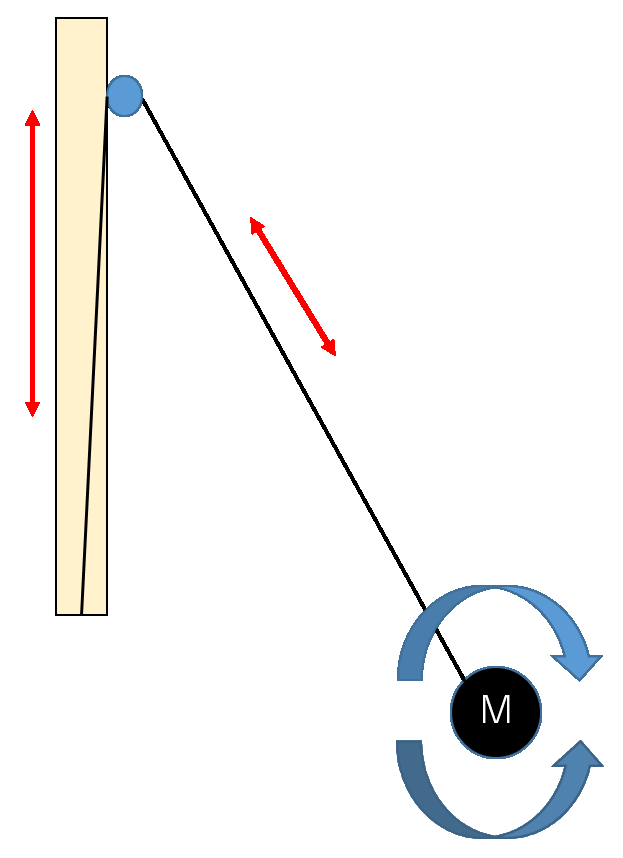
\includegraphics[clip,scale=0.4]{../../report_3/kakeru_report_03/picture/arm_img.eps}
   \caption{消火用アーム概念図}
 \label{arm_con}
\end{figure}



\begin{figure}[h]
 \centering
 \begin{tabular}{c}

  \begin{minipage}{0.3\hsize}
   \centering
   \includegraphics[clip,scale=0.05]{../../report_3/kakeru_report_03/picture/side_l.eps}
   \hspace{1.6cm} [1]アーム 左
  \end{minipage}

  \begin{minipage}{0.45\hsize}
   \centering
   \includegraphics[clip,scale=0.05]{../../report_3/kakeru_report_03/picture/side_r.eps}
   \hspace{1.6cm} [2]アーム 右
  \end{minipage}
 \end{tabular}
 \caption{消火用アーム}
 \label{arm_real}
\end{figure}
